\documentclass[14pt]{extarticle}
\usepackage{fontspec}
\usepackage{polyglossia}
\usepackage{amsmath}
\usepackage{amssymb}
\usepackage{xcolor}
\usepackage{fancyhdr}
\usepackage{graphicx}
\usepackage{listings}
\usepackage[most]{tcolorbox}
% \usepackage{setspace}
\usepackage{pifont}
\usepackage{enumitem}
\usepackage{titlesec}
\usepackage[bottom]{footmisc}
\usepackage{titling}
\usepackage{minted}
\usepackage{etoolbox}
\usepackage{array}
\usepackage{extsizes}
\usepackage{float}
\usepackage{booktabs}
\usepackage{hyperref}
\usepackage[onehalfspacing]{setspace}
\usepackage[a4paper, top=2.7cm, bottom=2.7cm, left=2.5cm, right=2.5cm, headheight=1.5cm, headsep=0.5cm]{geometry}
\usepackage{tikz}

\usetikzlibrary{automata, positioning, arrows.meta, arrows}

\newfontfamily\emoji{Segoe UI Emoji}

\pagestyle{fancy}

\setmainlanguage[numerals=western]{arabic}
\setotherlanguage{english}
% \newfontfamily\arabicfont[Script=Arabic]{Amiri}
\newfontfamily\arabicfont[Script=Arabic]{Calibri}
\newfontfamily\arabicfonttt[Script=Arabic]{Courier New}

\lstset{
  language=[Sharp]C,
  numbers=left,
  stepnumber=1,
  numbersep=8pt,
  frame=single,
  basicstyle=\ttfamily\small,
  keywordstyle=\color{blue},
  stringstyle=\color{red},
  commentstyle=\color{green!50!black}
}

\newif\ifdetailed
\ifdefined\setdetailed
  \setdetailed
\fi

\newif\ifwithsols
\ifdefined\setwithsols
  \setwithsols
\fi

% unified tcolorboxes for articles
\tcbset{colback=white, colframe=black, fonttitle=\bfseries, boxrule=0.8pt}
\newtcolorbox{boxDef}[1][]{colback=blue!5!white,colframe=blue!75!black,
  title={{\emoji📘} تعريف\ifx\\#1\\\else ~#1\fi :}}
\newtcolorbox{boxExercise}[1][]{colback=cyan!5!white,colframe=cyan!70!black,
  title={{\emoji🧩} تمرين\ifx\\#1\\\else ~#1\fi :}}
\newtcolorbox{boxExample}[1][]{colback=yellow!5!white,colframe=orange!90!black,
  title={{\emoji📝} مثال\ifx\\#1\\\else ~#1\fi :}}
\newtcolorbox{boxNote}[1][]{colback=gray!10!white,colframe=black,
  title={{\emoji✨} ملاحظة\ifx\\#1\\\else ~#1\fi :}}
\newtcolorbox{boxAttention}[1][]{colback=magenta!10!white,colframe=magenta!80!black,
  title={{\emoji🔔} تنبيه\ifx\\#1\\\else ~#1\fi :}}
\newtcolorbox{boxWarning}[1][]{colback=red!5!white,colframe=red!75!black,
  title={{\emoji⚡} ملاحظة هامة\ifx\\#1\\\else ~#1\fi :}}
\newtcolorbox{boxSolution}[1][]{colback=green!5!white,colframe=green!60!black,
  title={{\emoji✅} حل\ifx\\#1\\\else ~#1\fi :}}
\newtcolorbox{boxSymbol}[1][]{colback=purple!5!white,colframe=purple!70!black,
  title={{\emoji🔣} رمز\ifx\\#1\\\else ~#1\fi :}}
\newtcolorbox{boxHint}[1][]{colback=teal!5!white,colframe=teal!60!black,
  title={{\emoji💡} تلميح\ifx\\#1\\\else ~#1\fi :}}


\tcbset{simplecode/.style={ colback=gray!5, colframe=black!50, boxrule=0.4pt, arc=2pt, left=4pt,right=4pt,top=4pt,bottom=4pt}}
\newenvironment{boxCode}{\begin{tcolorbox}[simplecode]}{\end{tcolorbox}}

\newcolumntype{C}[1]{>{\centering\arraybackslash}p{#1}}

% redefine spaces after titles
\makeatletter
\renewcommand{\@maketitle}{%
  \begin{center}
    {\huge \bfseries \@title \par}%
    \vskip 0.2em % space between title and author
    {\large \@author \par}%
    % \vskip 0.2em % space between author and date
    % {\normalsize \@date \par}%
  \end{center}
}
\makeatother

\fancyhf{} % clear default
\fancypagestyle{plain}{
  \fancyhf{}
  \fancyhead[L]{مدرسة التسامح الشاملة}
  % \fancyhead[L]{
\includegraphics[height=1cm]{../../../images/logoTasamoh.png}}
  \fancyhead[R]{الأستاذ محمود اغبارية}
  \fancyfoot[C]{\thepage}
}

\fancyhead[L]{مدرسة التسامح الشاملة}
\fancyhead[R]{الأستاذ محمود اغبارية}
\fancyfoot[C]{\thepage}
% \date{\today}

\setcounter{tocdepth}{3} % only section subsection and subsubsection in TOC

\newcommand{\importpdfpage}[2]{%
    \thispagestyle{empty}
    \newgeometry{left=0cm,right=0cm,top=0cm,bottom=0cm}
    \includegraphics[page=#2,width=0.95\paperwidth,height=0.95\paperheight,keepaspectratio]{#1}
    \restoregeometry
}

\newcommand{\insertFullImg}[1]{%
    \noindent
    \makebox[\textwidth][c]{
        \includegraphics[width=0.9\paperwidth,keepaspectratio]{#1}%
    }%
}%

% ----------------------


% \begin{document}

% \maketitle

% % \clearpage  % start TOC on a new page
% % \renewcommand{\contentsname}{جدول المحتويات}
% % \tableofcontents
% % \clearpage

% \part*{part 1} % the * prevents numbering
% \section*{مقدمة}
% \subsection*{مثال رياضي}
% \subsubsection*{مثال فرعي}
% \paragraph*{ paragraph 1}
% \subparagraph*{sub paragraph 1}

% \ifdetailed
% \begin{english}
% \begin{minted}{csharp}
% // C# Example
% \end{minted}
% \end{english}
% \fi

% OLD WAY
% \ifdetailed
% \begin{english}
% \begin{lstlisting}
% // C# Example
% \end{lstlisting}
% \end{english}
% \fi

% % 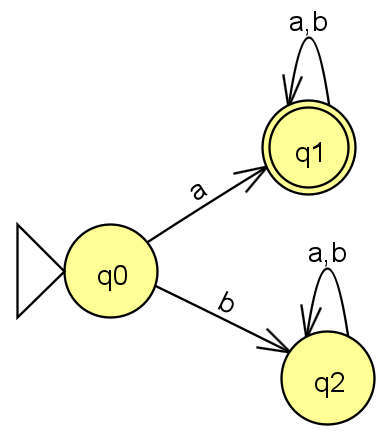
\includegraphics[width=0.2\textwidth]{../../../images/DFAs/ex1_q1.png}



% \vspace{3cm}
% \begin{flushleft}
% أرجو لكم وقتًا ممتعًا.

% الأستاذ محمود اغبارية.
% \end{flushleft}


% \end{document}


\ifwithsols
\title{حل ورقة تمرّن 18: مصفوفة كائنات}
\else
\title{ورقة تمرّن 18: مصفوفة كائنات}
\fi

\begin{document}

\maketitle
\thispagestyle{fancy}

جميع الأسئلة في هذه الورقة تعتمد على الفئة \textenglish{Student} التالية:

{\small
\begin{boxExample}
\begin{english}
\begin{minted}{csharp}
class Student
{
    private string Name;
    private int    ID;
    private double Grade;

    public Student(string name, int id, double grade)
    {
        this.Name  = name;
        this.ID    = id;
        this.Grade = grade;
    }

    public string GetName()  { return Name;  }
    public int    GetID()    { return ID;    }
    public double GetGrade() { return Grade; }

    public void SetGrade(double newGrade)
    {
        if (newGrade >= 0 && newGrade <= 100)
            Grade = newGrade;
    }

    public bool IsPassing()
    {
        return Grade >= 55;
    }

    public void Print()
    {
        Console.WriteLine($"[{ID}] {Name}: {Grade}");
    }
}
\end{minted}
\end{english}
\end{boxExample}
}
\clearpage

%=============================================================
\section*{الأسئلة}
%=============================================================

\begin{enumerate}

%-------------------------------------------------------------
\item % سؤال 1 — مراجعة: إنشاء كائنات في Main
%-------------------------------------------------------------

أنشئ في \textenglish{Main} ثلاثة كائنات من نوع \textenglish{Student} بالبيانات التالية، ثم اطبع كل منها باستخدام \textenglish{Print()}:

\begin{center}
\begin{tabular}{|c|c|c|}
\hline
\textbf{الاسم} & \textbf{الرقم} & \textbf{الدرجة} \\
\hline
\textenglish{Ali}  & \textenglish{101} & \textenglish{78.5} \\
\textenglish{Sara} & \textenglish{102} & \textenglish{91.0} \\
\textenglish{Omar} & \textenglish{103} & \textenglish{50.0} \\
\hline
\end{tabular}
\end{center}

\ifwithsols
{\small
\begin{boxSolution}
\begin{english}
\begin{minted}{csharp}
// In Main
Student s1 = new Student("Ali",  101, 78.5);
Student s2 = new Student("Sara", 102, 91.0);
Student s3 = new Student("Omar", 103, 50.0);

s1.Print();
s2.Print();
s3.Print();
\end{minted}
\end{english}
\end{boxSolution}
}
\clearpage
\fi

%-------------------------------------------------------------
\item % سؤال 2 — مراجعة: استخدام عمليات الفئة
%-------------------------------------------------------------

أنشئ كائنَين من نوع \textenglish{Student}:

\begin{english}
\begin{minted}{csharp}
Student s1 = new Student("Lina", 201, 48.0);
Student s2 = new Student("Nour", 202, 62.5);
\end{minted}
\end{english}

ثم اكتب كودًا يطبع لكل طالب رسالة تقول إن كان ناجحًا أم راسبًا، باستخدام العملية \textenglish{IsPassing()}.

\ifwithsols
{\small
\begin{boxSolution}
\begin{english}
\begin{minted}{csharp}
// In Main
Student s1 = new Student("Lina", 201, 48.0);
Student s2 = new Student("Nour", 202, 62.5);

if (s1.IsPassing())
    Console.WriteLine(s1.GetName() + " is passing.");
else
    Console.WriteLine(s1.GetName() + " is failing.");

if (s2.IsPassing())
    Console.WriteLine(s2.GetName() + " is passing.");
else
    Console.WriteLine(s2.GetName() + " is failing.");
\end{minted}
\end{english}
\end{boxSolution}
}
\clearpage
\fi

%-------------------------------------------------------------
\item % سؤال 3 — تعريف مصفوفة كائنات وطباعتها
%-------------------------------------------------------------

عرِّف في \textenglish{Main} مصفوفة \textenglish{students} من نوع \textenglish{Student} بحجم 4 عناصر، وملئها بالبيانات التالية، ثم اطبع جميع الطلاب باستخدام حلقة \textenglish{for}:

\begin{center}
\begin{tabular}{|c|c|c|}
\hline
\textbf{الاسم} & \textbf{الرقم} & \textbf{الدرجة} \\
\hline
\textenglish{Ahmad} & \textenglish{301} & \textenglish{85.0} \\
\textenglish{Dina}  & \textenglish{302} & \textenglish{73.5} \\
\textenglish{Yara}  & \textenglish{303} & \textenglish{90.0} \\
\textenglish{Karim} & \textenglish{304} & \textenglish{52.0} \\
\hline
\end{tabular}
\end{center}

\ifwithsols
{\small
\begin{boxSolution}
\begin{english}
\begin{minted}{csharp}
// In Main
Student[] students = new Student[4];
students[0] = new Student("Ahmad", 301, 85.0);
students[1] = new Student("Dina",  302, 73.5);
students[2] = new Student("Yara",  303, 90.0);
students[3] = new Student("Karim", 304, 52.0);

for (int i = 0; i < students.Length; i++)
    students[i].Print();
\end{minted}
\end{english}
\end{boxSolution}
}
\clearpage
\fi

%-------------------------------------------------------------
\item % سؤال 4 — عدّ العناصر في المصفوفة
%-------------------------------------------------------------

بافتراض وجود المصفوفة \textenglish{students} من السؤال السابق، اكتب كودًا في \textenglish{Main} يطبع:
\begin{itemize}
    \item عدد الطلاب الناجحين.
    \item عدد الطلاب الراسبين.
\end{itemize}

\ifwithsols
{\small
\begin{boxSolution}
\begin{english}
\begin{minted}{csharp}
// In Main
int passing = 0;
int failing = 0;

for (int i = 0; i < students.Length; i++)
{
    if (students[i].IsPassing())
        passing++;
    else
        failing++;
}

Console.WriteLine("Passing: " + passing);
Console.WriteLine("Failing: " + failing);
\end{minted}
\end{english}
\end{boxSolution}
}
\clearpage
\fi

%-------------------------------------------------------------
\item % سؤال 5 — إيجاد القيمة العظمى
%-------------------------------------------------------------

بافتراض وجود المصفوفة \textenglish{students}، اكتب كودًا في \textenglish{Main} يجد ويطبع الطالب صاحب أعلى درجة في المصفوفة.

\ifwithsols
{\small
\begin{boxSolution}
\begin{english}
\begin{minted}{csharp}
// In Main
Student best = students[0];
for (int i = 1; i < students.Length; i++)
{
    if (students[i].GetGrade() > best.GetGrade())
        best = students[i];
}

Console.Write("Top student: ");
best.Print();
\end{minted}
\end{english}
\end{boxSolution}
}
\begin{boxNote}
\textenglish{best} لا ينسخ الكائن — بل يُشير إليه. عند تحديث \textenglish{best} نحوّل الإشارة فقط.
\end{boxNote}
\clearpage
\fi

%-------------------------------------------------------------
\item % سؤال 6 — تعديل عناصر المصفوفة
%-------------------------------------------------------------

بافتراض وجود المصفوفة \textenglish{students}، اكتب كودًا في \textenglish{Main} يُضيف 5 نقاط لكل طالب راسب (درجته أقل من 55)، باستخدام \textenglish{SetGrade()}، ثم يطبع المصفوفة كاملةً بعد التعديل.

\ifwithsols
{\small
\begin{boxSolution}
\begin{english}
\begin{minted}{csharp}
// In Main
for (int i = 0; i < students.Length; i++)
{
    if (!students[i].IsPassing())
        students[i].SetGrade(students[i].GetGrade() + 5);
}

for (int i = 0; i < students.Length; i++)
    students[i].Print();
\end{minted}
\end{english}
\end{boxSolution}
}
\clearpage
\fi

%-------------------------------------------------------------
\item % سؤال 7 — عملية خارجية تتلقى مصفوفة كائنات
%-------------------------------------------------------------

اكتب عملية خارجية (\textenglish{static}) باسم \textenglish{PrintPassing} تتلقى مصفوفة \textenglish{Student[]} وتطبع فقط الطلاب الناجحين منها.

ثم استدعِها في \textenglish{Main} على مصفوفة \textenglish{students}.

\ifwithsols
{\small
\begin{boxSolution}
\begin{english}
\begin{minted}{csharp}
public static void PrintPassing(Student[] students)
{
    for (int i = 0; i < students.Length; i++)
    {
        if (students[i].IsPassing())
            students[i].Print();
    }
}

// In Main
PrintPassing(students);
\end{minted}
\end{english}
\end{boxSolution}
}
\clearpage
\fi

%-------------------------------------------------------------
\item % سؤال 8 — عملية خارجية تعيد مصفوفة كائنات
%-------------------------------------------------------------

اكتب عملية خارجية (\textenglish{static}) باسم \textenglish{GetTopStudents} تتلقى مصفوفة \textenglish{Student[]} وتُعيد مصفوفة جديدة تحتوي فقط على الطلاب الذين درجتهم أكبر من أو تساوي 80.

ثم استدعِها في \textenglish{Main} واطبع المصفوفة المُعادة.

\ifwithsols
\else
\begin{boxNote}
\textbf{تلميح:} مرّ على المصفوفة مرتين — مرة لحساب الحجم الصحيح للمصفوفة الجديدة، ومرة لملئها.
\end{boxNote}
\fi

\ifwithsols
{\small
\begin{boxSolution}
\begin{english}
\begin{minted}{csharp}
public static Student[] GetTopStudents(Student[] students)
{
    // First pass: count how many qualify
    int count = 0;
    for (int i = 0; i < students.Length; i++)
    {
        if (students[i].GetGrade() >= 80)
            count++;
    }

    // Create result array of exact size
    Student[] result = new Student[count];

    // Second pass: fill result array
    int j = 0;
    for (int i = 0; i < students.Length; i++)
    {
        if (students[i].GetGrade() >= 80)
        {
            result[j] = students[i];
            j++;
        }
    }

    return result;
}

// In Main
Student[] top = GetTopStudents(students);
for (int i = 0; i < top.Length; i++)
    top[i].Print();
\end{minted}
\end{english}
\end{boxSolution}
}
\fi

\end{enumerate}

\ifwithsols
\else
\vspace{1em}
\begin{flushleft}
أرجو لكم عملاً ممتعاً!

الأستاذ محمود اغبارية
\end{flushleft}
\fi

\end{document}
